% $Id$
% cpp-aware-c-analyses.tex

%% TODO:
% package and put code up at ftp site
% add personal.sty package
% get references in the right order
% any grants to add?
% new astlog-example-inspired section?  see FIXME
% floppies
% see authors notes
% sign publishing agreement


%\documentclass[twocolumn]{article}
\documentclass{article}
%\usepackage{icse99}
\usepackage{fullpage}
\usepackage{graphicx}
\usepackage{rotating}
\usepackage{lscape}
%\usepackage{personal}

\renewcommand{\baselinestretch}{2}
\newcommand{\B}{\discretionary{}{}{}}

%%% Some stuff from Mike
%%% Figures
%%%

%% Get a line between figures at the top of the page and the text
\makeatletter
\def\topfigrule{\kern3\p@ \hrule \kern -3.4\p@} % the \hrule is .4pt high
%\def\botfigrule{\kern-3\p@ \hrule \kern 2.6\p@} % the \hrule is .4pt high
\makeatother

%% This is too crowded...
% \setlength{\textfloatsep}{0.25\textfloatsep}
% \setlength{\dbltextfloatsep}{0.25\dbltextfloatsep}
%% ...but I can live with halving it (still a bit crowded for my taste).  -MDE
\setlength{\textfloatsep}{0.5\textfloatsep}
\setlength{\dbltextfloatsep}{0.5\dbltextfloatsep}

%% Permit text to appear on pages containing many big figures
\def\floatpagefraction{.8}      % default .5
\def\textfraction{.2}
\def\topfraction{.8}

%%% End stuff from Mike

\newcommand{\pcp}{\mbox{\textsf{PCp}$^3$}}
\newcommand{\pcppp}{\mbox{\textsf{PCppP}}}
\newcommand{\Cpp}{\mbox{\textsf{cpp}}}
%\newcommand{\CPP}{\mbox{\textsf{C\texttt{++}}}}
\newcommand{\CPP}{\mbox{C\texttt{++}}}
%\newcommand{\Perl}{\mbox{\textsf{Perl}}}
\newcommand{\Perl}{\mbox{Perl}}
%\newcommand{\C}{\mbox{\textsf{C}}}
\newcommand{\C}{\mbox{C}}

\newcommand{\backcall}[3]{\item \texttt{#2} (\texttt{#3})
  \ifthenelse{\equal{#1}{}}{}{\textbf{returns} \texttt{#1}} \\ }

%\newcommand{\backcallobsoleted}[3]{\item \texttt{#2} (\texttt{#3})
%  \textbf{returns} \texttt{#1} \textsc{Obsoleted}\\ }

% Don't even print these out for the paper
\newcommand{\backcallobsoleted}[3]{}

\newcommand{\hook}[2]{\texttt{#1}(\texttt{#2}) \\ }
\newcommand{\shook}[1]{\texttt{#1}}

\newcommand{\hookobsoleted}[2]{}
\newcommand{\pphash}{\texttt{\#}}

\newcommand{\ppd}[1]{\texttt{\##1}}

\newcommand{\file}[1]{{\small \texttt{#1}}}
\newcommand{\email}[1]{{\small \texttt{#1}}}
\newcommand{\program}[1]{{\small \texttt{#1}}}
\newcommand{\syscall}[1]{{\textsf{#1}}}
\newcommand{\sectionref}[1]{section \ref{#1}, on page \pageref{#1}}
\newcommand{\appendixref}[1]{Appendix \ref{#1}, on page \pageref{#1}}
\newcommand{\ie}{i.e.,}
\newcommand{\eg}{e.g.,}
\newcommand{\etc}{etc}  % trailing ".\ " needed at use; this just for
                        % italicizing optionally
\newcommand{\figref}[1]{Figure~\ref{#1}}
\setlength{\fboxsep}{.1in}

\title{A Framework for Preprocessor-Aware \\ C Source Code Analyses}
\author{
        \hspace*{-2ex}
        \parbox{4in} {\begin{center}
        Greg J. Badros and David Notkin\\
        \end{center}}\\
        \parbox{4in} {\begin{center}
            \begin{small}
              Dept. Computer Science \& Engineering\\
              University of Washington \\
              Box 352350, Seattle WA  98195-2350 ~ USA \\
              +1-206-543-1695\\
              \email{\{gjb,notkin\}@cs.washington.edu}
            \end{small}
        \end{center} }
}

%\date{31 January 1999}
%\date{27 June 1999}
%\date{14 July 1999}
\date{14 November 1999}


\begin{document}
\maketitle
% \copyrightspace
%\submitspace{\LARGE{Draft of paper\\ submitted to ICSE 99.}}

\thispagestyle{empty}  % suppresses page number on first page

\pagestyle{plain}

\section*{Abstract}
\label{sec:abstract}
Analyses of \C{} source code usually ignore the \C{} preprocessor
because of its complexity.  Instead, these analyses either define their
own approximate parser or scanner or else they require that their
input already be preprocessed.  Neither approach is entirely
satisfactory: the first gives up accuracy (or incurs large
implementation costs), while the second loses the preprocessor-based
abstractions.  We describe a framework that permits analyses to be
expressed in terms of both preprocessing and parsing actions, allowing
the implementer to focus on the analysis.  We discuss an implementation of
such a framework that embeds a \C{} preprocessor, a parser, and a Perl
interpreter for the action ``hooks.''  Many common software engineering
analyses can be written surprisingly easily using our implementation,
replacing numerous ad-hoc tools.  The framework's integration of the
preprocessor and the parser further enables some analyses that otherwise
would be especially difficult to perform.

\subsection*{Keywords}
Parsing, preprocessor, C, lexical analysis, syntactic analysis, Perl.

\bigskip

% Introduction, including problem statement, goals, etc
\section*{Introduction}
\label{sec:intro}
More than twenty years ago, Dennis Ritchie designed the \C{}
language~\cite{Kernighan88} to include a textual macro preprocessor
called \Cpp{}~\cite[Ch.~3]{Harbison91}.  Given the simplicity of the
language and the state of the art in compiler technology in the
mid-1970s, his decision to provide some language features in this
extra-linguistic tool was justified.  For the last two
decades, \C{} programs have exploited \Cpp{}'s capabilities for
everything from manifest constants and type-less pseudo-inline
functions to modularization and symbol generation.  Bjarne
Stroustrup, the designer and original implementor of \CPP{}, notes that
``without the \C{} preprocessor, \C{} itself $\ldots$ would have been
stillborn''~\cite[p.~119]{Stroustrup94}.  Certainly \Cpp{} contributes
to \C{}'s expressiveness and portability, but perhaps at too large a
cost.  Stroustrup recognizes this tradeoff:

\begin{quotation}
\noindent Occasionally, even the most extreme uses of \Cpp{} are useful, but its
facilities are so unstructured and intrusive that they are a constant
problem to programmers, maintainers, people porting code, and tool
builders~\cite[p.~424]{Stroustrup94}.
\end{quotation}

\subsection*{Why \Cpp{} is good $\ldots$ \emph{and} bad}

The intrinsic problem with \Cpp{} is also its fundamental strength: it
is a distinct first pass of textual (non-syntactic) processing over the
source code.  This introduces significant differences between the code
that the programmer sees and what the compiler proper (\ie{} the \C{}
compiler distinct from the preprocessor) ultimately
compiles.\footnote{To avoid ambiguity, we will use \emph{unprocessed} to
  refer to the original source code, and \emph{preprocessed} to refer to
  the view of the code after running \Cpp{} on it.}

Experienced and novice \C{} programmers alike are frustrated by
misunderstandings of source code due to the arbitrary transformations
\Cpp{} performs. A software engineer might want to be sure that a
function \texttt{foo} is not invoked in a given block of code.  By
simply visually scanning that code segment, though, she may be oblivious 
to a seemingly-unrelated macro that happens to expand to an invocation
of \texttt{foo}, the function intended to be avoided.

Such confusions are easily reduced, if not eliminated,
by allowing the software engineer to see the code exactly as the
compiler does.  Unfortunately, that view of the program is at a level of
abstraction lower than the unprocessed source.  Well-known
identifiers such as \texttt{stderr} may appear as the far less readable
\texttt{(\_IO\_FILE*)(\&\_IO\_stderr\_)},
%\footnote{This is the
%  output generated when preprocessed using the \texttt{gcc} compiler's
%  standard include files.}
and useful encapsulations such as \texttt{assert} degenerate into
sequences of symbols that are less meaningful to a human programmer.  Every
non-trivial \C{} program uses the preprocessor, and an empirical study
of numerous packages written in \C{} documents the extensive use of \Cpp{}
constructs~\cite{EmpCpp-TR}.

Though \Cpp{} is sometimes used by other languages (\eg{}
\texttt{Java} programs and the X11 \texttt{xrdb} resource database
language) and causes similar difficulties whenever used, we focus on
\Cpp{}'s use with \C{} code exclusively.  We are interested in the huge
body of \C{} programs, and helping programmers understand and extend
those software artifacts. \Cpp{} is a necessary and integral part of the
\C{} programming language specification.  In practice, the \C{}
preprocessor is almost never separated from \C{} code, thus the issues
relating the \Cpp{} arise with virtually all \C{} programs.  Though we
focus on \C{}, the framework we describe could be applied to analyze other
uses of \Cpp{} (and even other textual preprocessing languages) in a
fairly direct way.


%Unlike syntax-based macros~\cite{Weise93} which operate at the parser
%level, \Cpp{} provides macros and conditional inclusion mechanisms which
%operate at the lexical level.  The \C{} preprocessor also includes
%``stringization'' and pasting operators which manipulate symbols
%directly, altering their ultimate interpretation by a parser.  

\subsection*{\Cpp{} and Software Tools}

Because of the preprocessor's textual foundations, unprocessed \C{} source code
cannot be parsed directly.  For example, identifiers that are macro-expanded may
hide braces, parentheses, or other 
important tokens from the parser.  Only after preprocessing is a \C{} program
in a grammatically usable form. Since parsing
preprocessed code is relatively easy and well-understood,
most software engineering tools operate on
exactly that view of the source, losing abstractions that are
expressed in \Cpp{}.  

Various tools including source-level debuggers and call graph extractors
either run \Cpp{} as the first stage in their analysis, or use
representations derived from a compiler operating on the preprocessed
code.  For example,
Siff and Reps implement a function-generalization transformation
tool that operates on preprocessed code, but note that future versions
of their tool must drop that requirement so that macro abstractions are
not lost~\cite{Siff96}. Using preprocessed code for program
understanding or transformation tasks is fraught with difficulties due
to changes in the source artifact from preprocessing.\footnote{In
  contrast, this approach is exactly right for the compiler, where there is
  no need to preserve high level abstractions while generating object
  code.}

%  However, in the presence of errors, the compiler itself is a
%  program-understanding tool and preprocessing hinders its ability to
%  accurately describe the problem.  The automatically output \ppd{line}
%  directive provides a rudimentary (but far too coarse)
%  mapping to the original source to permit better diagnostics.}

% Additionally, parsing requires a syntactically correct program with all
%header files present---often unrealistic constraints during 
% software maintenance activities such as porting or switching
% compilers.
% -- above point isn't something that our system fixes --08/25/98 gjb
Another disadvantage of preprocessing is that it eliminates
conditional compilation directives that are essential to the portability
and versatility of the source code~\cite{Krone94}.  Preprocessing
forces tools to limit their analysis to a single configuration of the
source code, instead of permitting global reasoning about the entire
artifact.  

Some tools instead operate on the
unprocessed source code exactly as the programmer sees it.  This
technique improves robustness in handling syntax errors
and language variants. Because the input is unprocessed, the extracted
information is presented to the human software engineer at the same
level of abstraction as the source.  Additionally, the unprocessed
source still contains the preprocessor directives that are essential
to the portability and flexibility of many \C{} programs.

However, these tools cannot use a straightforward parser or reliably construct an
abstract syntax tree because the source is not
grammatically-correct \C{} code.  Lexical tools such as \texttt{etags},
LSME~\cite{Murphy96}, and \texttt{font-lock-mode} for Emacs and
approximate parsers such as \texttt{Field}~\cite{ReissField} and
\texttt{LCLint}~\cite{LCLint} use this approach.  However,
disregarding or only partially honoring the \Cpp{} directives leads to
an extracted model of the source code that is only an approximation of
the program's appearance to a compiler.  Certain uses of the
preprocessor can cause substantial problems:  the syntax of declarations 
or scoping constructs can be customized and arbitrary code can be hidden in macro
expansions.  Macro expansion was a
major cause of both false positives and false negatives in call graph
extraction~\cite{Griswold96}.  Such approximate tools are inappropriate
for software engineering analyses that require exact or conservative
information.

We introduce a new approach that integrates the \C{} preprocessor and a
parser in a flexible framework for statically analyzing \C{}
source code.  The framework makes it easy for tool builders to produce
analysis tools for \C{} source code that are capable of reasoning about the
preprocessor.


%  Section~\ref{sec:framework} describes that framework and
%illustrates a sample analysis (a call-graph extraction) using the
%framework.  Section~\ref{sec:further_examples} details a pair of
%macro-expansion understanding analyses, and section~\ref{sec:pcp3} describes our
%prototype tool, \pcp{}. Finally, section~\ref{sec:related} discusses
%related work, and sections~\ref{sec:limitations} and \ref{sec:conclusion}
%review the limitations of our approach and conclude.

\section*{The Framework}
\label{sec:framework}

The idea behind our framework is simple: provide an integrated parser
and preprocessor that controls the scanning of the source code while
executing user-defined callbacks when specified ``interesting'' actions occur.
Though similar to the way the \texttt{yacc} parser~\cite{Levine92}
associates actions with parse rule invocation, our framework provides
callbacks on both parser and preprocessor actions. Additionally,
instead of \C{} as the language for the actions, we use the \Perl{} scripting
language for writing the hook subroutines.  Griswold, Atkinson and McCurdy note
that various software tools benefited from using a special-purpose
action language~\cite{Griswold96}, and interpreted languages can
often significantly speed development time~\cite{Scripting}.
Additionally, \Perl{} is sufficiently similar to \C{} that it is easy to 
learn by \C{} programmers.  \Perl{} also provides closures which make
expressing and registering the callback routines very concise and
readable. The nearly-immediate turn-around time that
\Perl{} provides is especially useful when prototyping and debugging new 
analyses.  Our prototype implementation of the framework is called
\pcp{}, pronounced ``pee-see-pee-cubed.''


Callbacks can be installed on actions such as the scanning of preprocessor directives, the
creation of a macro definition, the expansion (\ie{} use) of a macro
name, and the parsing of a variable declaration.  Each action callback
is passed arguments relevant to the event for which it was invoked.  For
example, the \texttt{TYPEDEF} action receives the name of the declared
type as its first argument.  See the first appendix
%~\ref{sec:hooks} 
for a more complete list of the hooks in our current implementation of
the framework.

To supplement the directly-passed arguments, action subroutines may also invoke
``backcalls'' to access internal
parser and preprocessor data structures. Example backcalls include
getting the name of the currently-processed file, looking up a symbol in
the parser's symbol table, inserting arbitrary code for the preprocessor
to process, and instructing the parser to enter a new scope. 
See the second appendix
%Appendix~\ref{sec:backcalls} 
for a more complete list of
the backcalls in our current implementation of the framework.

The callback and backcall interfaces combined with a general
purpose scripting language provide a concise and flexible means for
easily writing static analyses of \C{} source code.  The framework
itself is extensible with additional callbacks and backcalls by
re-compiling the analysis tool after inserting the new callback
invocations and backcall functions.  Extending the framework is intended 
to be a far less frequent need than using the framework to perform a new 
analysis, so the additional developer time in writing, compiling, and
testing C code extensions is acceptable.


%\begin{figure*}[t]
\begin{figure*}[p]
\begin{center}
\begin{small}
\begin{pseudocode}[5.5in]
use pcp3;
my %func_calls = ();  # the dictionary of callees for the current function
                      # maps called function name to number of times in appears
                      #   in the definition of the calling function

AddHook("FUNC_SPEC", sub { %func_calls = (); } );
AddHook("FUNC_CALL", sub { # $_[0] argument is the name of function invoked
                           $func_calls{$_[0]}++; } );
AddHook("FUNCTION", 
   sub { # $_[0] argument is the name of function just defined
     if (scalar (keys %func_calls) > 0) {
       print "$_[0] calls ", join(", ", sort keys %func_calls), "\n";
     }
   } );
\end{pseudocode}
\end{small}
\caption{A complete static analysis to extract a call graph.}
\label{fig:call_graph_extractor}
\end{center}
\end{figure*}
%$

\subsection*{Example: Call-Graph Extraction}
\label{sec:call_graph_extraction}


One common software engineering analysis is to extract a call graph from a
body of \C{} source code.  Our framework permits this analysis to be
written in about ten lines of code, as shown in
Figure~\ref{fig:call_graph_extractor}.

To perform the analysis, we attach subroutines to three parsing
callbacks.  When a function specifier (that is, 
the signature specification of a
function definition) is parsed, the \texttt{FUNC\_SPEC} hook is
activated.  That callback resets the set of functions invoked by
the current function.  For each function call parsed, the
\texttt{FUNC\_CALL} hook is activated, and we add the name (passed to
the subroutine as the zeroth argument) of the called function to the
set.  Finally, when the entire function definition has been parsed, the
\texttt{FUNCTION} reduction occurs and we output the set of called
functions we accumulated while scanning the body of the function
definition.

The script does not implement the main control flow of the
analysis.  Also, it need not handle any preprocessor directives.  Since
this simple analysis deals only with parser actions, the view the
analysis sees is exactly the same as if we had analyzed the preprocessed 
code.

\subsection*{Revising the Extractor}
\label{sec:call_graph_revised}
The simple call-graph extractor used as an example in the preceding
section suffers from many of the same shortcomings as tools that
operate on preprocessed code: it reasons about only a single
configuration of the source and eliminates all macro abstractions
from the extracted model.  As Murphy et al.\ discuss, there are many
degrees of freedom for call-graph extractors~\cite{Murphy98}.  As
written, the analysis counts all function calls in macro expansions as
occurring from the function in which the macro is expanded---the macro
expansion itself is omitted from the call graph.  This behaviour may not 
always be what the software engineer desires. However, a substantial
strength of our framework is that it lets a tool-builder easily
fine-tune the extraction to derive the desired view.

For example, often macros are used to express inline functions.  If we
choose, we can have macro expansions included in the extracted
call-graph:

\begin{verbatim}
# $_[2] is the macro name being expanded
AddHook("EXPAND_MACRO", 
     sub { $func_calls{$_[2]}++; }
\end{verbatim}
%$

\noindent Given this revised extractor, a macro that expands into code
that includes function calls will expose those function calls as callees
from the function definition in which the macro was expanded.  For some
tasks, this may be exactly what we want.  If instead we prefer to hide
those nested calls, our framework supports that behaviour as well.  We
simply ignore function calls that we parse while expanding macros (see
Figure~\ref{fig:rev_call_graph_extractor}).

Another possible extension of the analysis is to query the symbol table
for the type of the identifier being called.  If the variable is a
pointer to a function, the enclosing function could conservatively be
marked as ``possibly calling all functions'' (\ie{} $\bot$).\footnote{A more
aggressive analysis could maintain data on which functions
are ever assigned to the variable throughout the program.}

%\begin{figure*}[hbt]
\begin{figure*}[p]
\begin{center}
\begin{small}
\begin{pseudocode}[5.5in]
use pcp3;
my %func_calls = ();  # the set of callees for the current function
my $expanding = 0;    # are we expanding a macro?

AddHook("FUNC_SPEC", sub { %func_calls = (); });
AddHook("FUNC_CALL", sub { # $_[0] argument is the name of function invoked
                           $func_calls{$_[0]}++ if !$expanding; } );
AddHook("EXPAND_MACRO", sub { # $_[2] argument is macro name being expanded
                              $func_calls{$_[2]}++ if !$expanding; 
                              ++$expanding} );
AddHook("MACRO_CLEANUP", sub { --$expanding; } );

AddHook("FUNCTION", 
  sub { # $_[0] argument is the name of function just defined
    if (scalar (keys %func_calls) > 0) {
      print "$_[0] calls ", join(", ", sort keys %func_calls), "\n";
    }
  } );
\end{pseudocode} %$
\end{small}
\caption{A revised call graph extractor that treats macros as functions.}
\label{fig:rev_call_graph_extractor}
\end{center}
\end{figure*}

Because the activations of the preprocessor and parser hooks
are intermingled, the analysis can reason about the preprocessed version 
of the source within the context of how it was preprocessed.  

\subsection*{Preprocessor and Parser Interactions}
\label{sec:interactions}

Given a straightforward preprocessor and parser front end, some analyses
are impossible.  For example, since the preprocessor will skip code as
instructed by conditional compilation directives, that source will be
left unprocessed. If our analysis is intended to find all invocations
of a function, we will often want conditional-compilation branches that
are unused for the current platform to still undergo the analysis (as
they would by a lexical tool such as \texttt{grep}, but unlike the
behaviour achieved by operating on preprocessed code).

To permit handling the otherwise-skipped code hidden by conditional
compilation directions such as \ppd{ifdef} and \ppd{if}, our framework
provides a general mechanism for inserting arbitrary source text to be
processed.  Action subroutines can pass a string to the \texttt{PushBuffer}
backcall.  A hook, \texttt{DO\_XIFDEF}, is called for all conditional
compilation directives and provides an argument that is the text that
would \emph{not} be included.  The action routine for that hook may then
use \texttt{PushBuffer} to ask the preprocessor and parser to use that
string as input and process it normally.

However, since such program text can include arbitrary preprocessor
directives and \C{} code, we may want to ensure that the state of
neither the preprocessor nor the parser is permanently changed after the
``for analysis only'' parsing of the skipped code.  Three data
structures must be preserved to avoid side-effects to the main
processing (\ie{} the version selected by the \ppd{define}dness of macro
names): the preprocessor's hash table of macros, the \C{} symbol table,
and the parser's current stack of states.  

The backcalls \texttt{PushHashTab} and \texttt{PopHashTab} save and
restore the preprocessor's table of definitions so that preprocessor
directives in skipped code will not affect \Cpp{} when normal processing
resumes.  For the symbol table, the backcalls \texttt{EnterScope} and
\texttt{ExitScope} provide similar functionality.  Finally,
\texttt{YYPushStackState} and \texttt{YYPopStackState} save and restore
the stack of parser states.  In under fifty lines of boiler-plate code,
an analysis tool can manage these complexities and expose the full source to
the analysis.  This template code is included with \pcp{}.

Other related backcalls provide additional support for querying and
interacting with the parser.  \texttt{ParseStateStack} returns the
list of states in the parser's stack; this exposes information about what
constructs might be legal at the current location (for example,
determining whether declarations may be permitted).
\texttt{SetStateStack} permits explicitly changing the parser's stack
of states, perhaps to prepare for handling a top level construct or to
re-parse text using a different configuration of the parser.  Using
\texttt{YYFCompareTopStackState}, an action hook can efficiently check
whether a previously saved parser state matches the current
configuration.  For example, an analysis can easily provide a warning
whenever the ``if'' block and the ``else'' block of an \ppd{ifdef}
directive leave the parser in different states.

One minor complexity with analyzing both paths of a conditional
compilation directive involves the \ppd{include} directive.  Often
header files that might recursively include themselves are protected
against entering an infinite inclusion loop by being enclosed in an
\ppd{ifndef} that skips the entire file when re-included:

\begin{verbatim}
#ifndef FOO_H__
#define FOO_H__

/* body of foo.h header */
#include "header-that-includes-foo.h"

#endif
\end{verbatim}

If an analysis were always to evaluate the code inside the \ppd{ifndef},
it would repeatedly and inifinitely re-analyze \file{foo.h}.  To avoid
this difficulty, an analysis can simply choose to not include a header file more
than once.  The \texttt{DO\_INCLUDE} callback permits the software
engineer to return \texttt{FALSE} to signify that the inclusion
directive should be ignored.  If an analysis is using
\texttt{PushBuffer} to process code that would otherwise be skipped,
then only the first attempt to include a given file should be allowed:

\begin{verbatim}
sub do_include { 
  my (undef,undef,undef,$file_as_resolved,undef) = @_;
  return FALSE if ($already_included{$file_as_resolved});
  $already_included{$file_as_resolved} = $true;
  return TRUE;  # permit the inclusion
}
\end{verbatim}

Once the file is included, the analysis continues from the new file.
When that file is completely analyzed, the \texttt{DONE\_INCLUDE\_FILE}
callback is invoked.  This permits the analyses to track file inclusions 
and perform any necessary cleanup or per-header-file processing.

% Possible applications
%** Tags generation
%** parser debugging, teaching
%** multi-version reasoning

\section*{Further Examples}
\label{sec:further_examples}

Preprocessor-specific analyses are generally especially difficult to
write.  The complexities and subtleties of \Cpp{} must be duplicated in
each tool.  Not surprisingly, our framework is ideal for analyzing
preprocessor constructs.

\subsection*{Macro Expansion Mappings}
\label{ssec:macro_exp_map}
To support useful interactions between the parser and preprocessor, it
is essential that \pcp{} maintain an accurate mapping between the
unprocessed source and the preprocessed source.  Macro expansions are
the most complicated aspect of this correspondence.  Macro arguments can
themselves be macros, and macros can expand to other macros in need of
expansion.\footnote{In ANSI \C{}'s preprocessor, recursion is
  prohibited; as a macro name is expanded, that name is disabled from
  future expansions generated by the original expansion.}  To
effectively exploit the macro expansion hooks, the details of the
expanding and substituting process must be understood.  For
\texttt{gcc}'s preprocessor, and consequently for \pcp{}, macro
expansion takes place as follows:\footnote{This description is necessarily
  implementation specific.  The \C{} language standard provides details
of what is required \cite[Ch.~3]{Harbison91}.  Also note that
  details of stringization and pasting are omitted as they are
  infrequently used features~\cite{EmpCpp}.}

\begin{enumerate}
\item The macro definition's body is checked to see which arguments it uses.
\item Those actual arguments that are used in the definition body are
      expanded if and only if they contain macros.  They are expanded
      completely (\ie{} macros in their expansions are expanded), and
      the text of the expansion is saved.  Identical arguments are
      expanded independently; for example \texttt{FOO(BAR,BAR)} will
      expand \texttt{BAR} twice if the expansion of \texttt{FOO} uses
      both of its arguments.  They are expanded in the order that they
      syntactically appear in the body of the expansion (not from first formal
      argument to last).
\item The body of the top level macro is copied left to right; arguments
      are replaced with the text from their expansions.  Macro names
      previously expanded are escaped (using a prefix of the
      distinguished symbols ``\texttt{@-}'') in this pseudo input buffer
      to prevent recursion.
\item That entire text is rescanned, and un-escaped macros are expanded
      further.
\end{enumerate}

\noindent The \texttt{EXPAND\_MACRO} hook is called for each macro name as it is
expanded.  The parameters to the hook include the exact location of the
start and end of the macro invocation in the source code.\footnote{Or,
  if the invocation does not directly appear in the source (\ie{} the
  macro appears in the expansion of another macro), the location is an
  offset within the prior macro's expansion.}  Other parameters
describe the ``nesting'' of the expansion, and a backcall
\texttt{Macro\-Expansion\-History()} describes the current history of
expansions.  The nesting of an expansion is the trail through arguments
of other macros that led to this expansion, while the expansion history
is a list of macros that were expanded en route to this macro being
expanded.

\begin{figure}[p]
  \begin{center}
    \leavevmode
    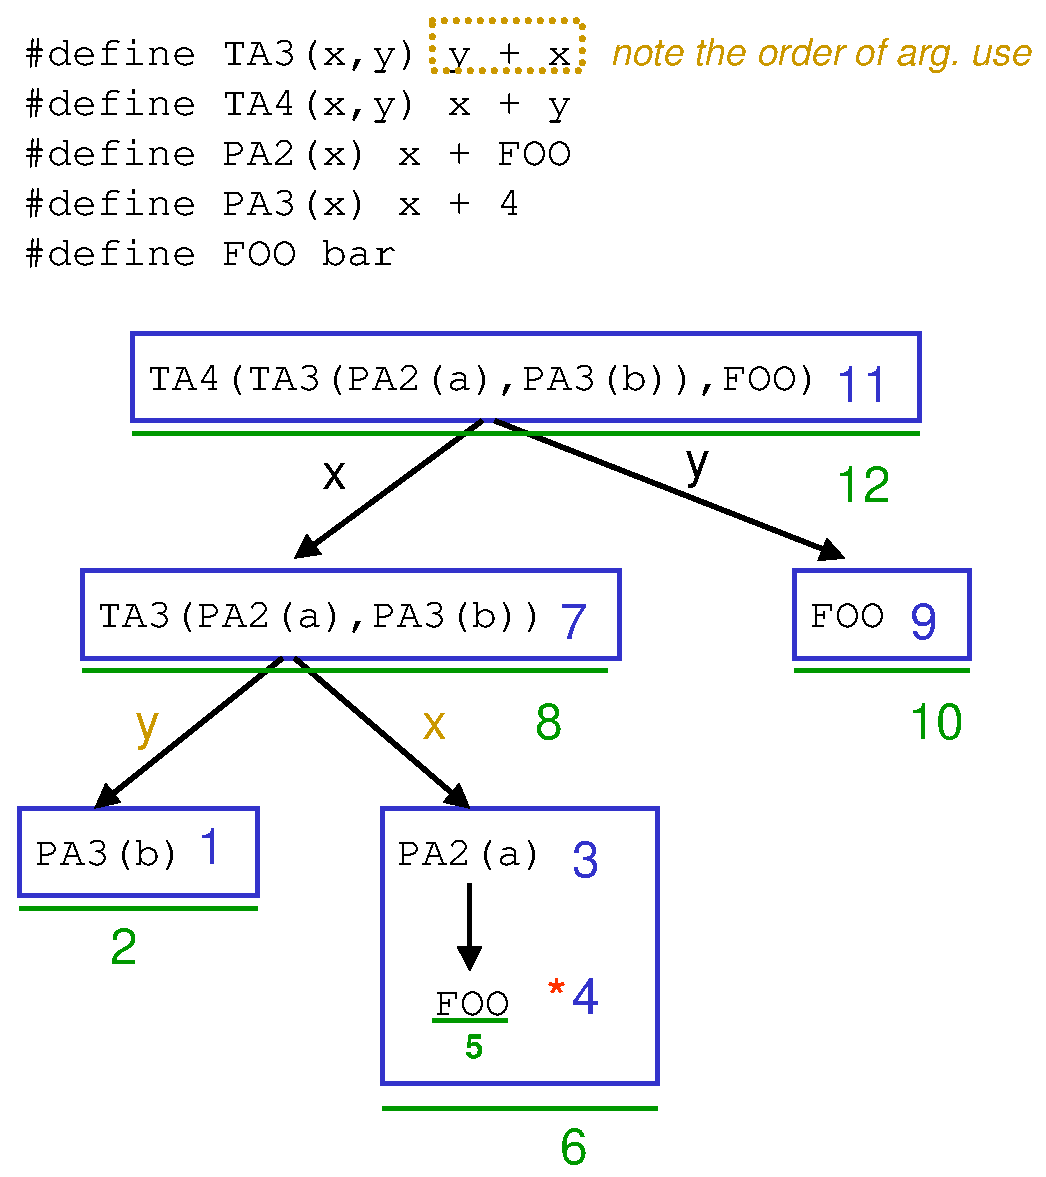
\includegraphics[width=0.45\linewidth]{tree-expn.eps}
    \caption{An example macro expansion and the related
      hooks that are called. Numbers indicate the order in which the
      hooks are called (corresponding to post-order traversal of the
      tree). Blue numbers are \texttt{EXPAND\_MACRO} actions, green
      numbers are \texttt{MACRO\_CLEANUP} actions; \eg{} the fifth hook
      \pcp{} invokes is \texttt{MACRO\_CLEANUP} for ``\texttt{FOO}''.
      The ``cleanup'' means that the macro has been fully expanded and
      is ready to be substituted into the output text (or parsed by
      \pcp{}). In general, the tree need not be
      binary. Note that the leaves of a node are the arguments in the
      order of appearance in that node's macro expansion (not their
      order in the list of formal parameters).}
    \label{fig:tree-expn}
  \end{center}
\end{figure}

\begin{figure}[p]
  \begin{center}
    \leavevmode
    \includegraphics[width=0.45\linewidth]{text-expn.eps}
    \caption{Another view of an example macro expansion and the hooks
    that are called.  Red dotted lines are the nestings of macro
    expansions as the algorithm recurses.  Blue lines are
    \texttt{EXPAND\_MACRO} actions on the underlined macro invocation,
    green lines are \texttt{MACRO\_CLEANUP}s.}
    \label{fig:text-expn}
  \end{center}
\end{figure}

Consider the example illustrated in figures \ref{fig:tree-expn} and
\ref{fig:text-expn}.  When the \texttt{MACRO\_EXPAND} hook is called for
\texttt{FOO} (marked with an asterisk in the figures), we have:

\begin{verbatim}
   @nests                   == ( TA3#1; TA4#1 )
   MacroExpansionHistory()  == ( PA2#Body )
\end{verbatim}

\noindent The \texttt{@nests} list tells us we are expanding the first
argument of macro \texttt{TA3}, which itself was the first argument of
macro \texttt{TA4}.  The \texttt{MacroExpansionHistory()} backcall
provides the remaining information about this expansion: that the
expansion came from the body of the earlier expansion of macro
\texttt{PA2}.  From \figref{fig:text-expn}, the \texttt{@nests} list
for a given expansion corresponds to the sequence of red dotted lines
directly above and completely overlapping the blue line representing
that expansion.  Similarly, the list \texttt{MacroExpansionHistory()}
returns can be visualized as the stack of blue expansion
lines directly above the expansion in question (those that have not
already been paired with a green line representing the completion of
their expansion).  

%% Emacs support
%\subsection*{Program understanding support in Emacs}
%\label{ssec:prg_und_supp}
This macro-expansion analysis generates a large amount of
information that is not easy to comprehend in raw form. 
To support visualizing these data we provide a
\Perl{} module of hook utilities that 
outputs character-indexed annotations of the source code.
These annotations are Emacs Lisp source code that manipulate text
properties of character ranges when evaluated by Emacs~\cite{GNUELisp}.
As the cursor is moved over source code
that has been annotated, a subsidiary Emacs frame dynamically displays
the annotations made to the current character. See
~\figref{fig:emacsdocprop} for an example.

%\begin{figure}[b!]
\begin{figure}[p]
  \begin{center}
    \leavevmode
    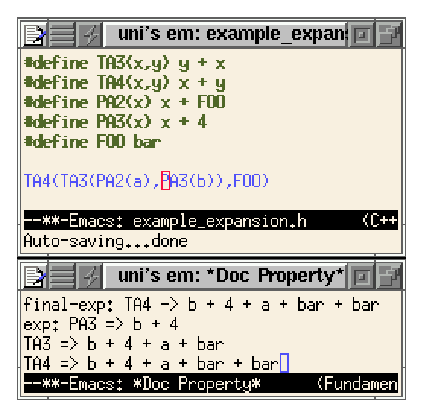
\includegraphics{emacs-xform-view.eps}
    \caption{A view of Emacs using the authors' ``doc-property-display''
      feature to dynamically view textual annotations of results of the
      analyses of \pcp{}.  The outline box in the top frame
      indicates the user's cursor position, and the lower frame lists the
      various text properties attached to the character there.
      The bottom frame potentially changes after each cursor movement.}
    \label{fig:emacsdocprop}
  \end{center}
\end{figure}


Annotating text makes more sense than annotating the abstract syntax
tree for several reasons.  First, \Cpp{} operates at a textual level.
As we have seen, the unprocessed source code cannot necessarily be
viewed as an ordinary abstract syntax tree.  Even if a generalized tree
could be constructed, no available interface provides adequate means
of interacting with the large, complicated trees that inevitably result
from realistic packages.
%~\footnote{The intentional programming group at
%  Microsoft Research is actively investigating this
%  area~\cite{MSIPPersonal}.}  
Additionally, text permits using Emacs as the target interaction
environment. This allows software engineers to augment Emacs's other
powerful source code understanding tools (\eg{} \texttt{font-lock-mode},
\texttt{etags}, \texttt{OOBrowser}, \etc{}.)  with their own annotations
supplied by \pcp{} analyses.



\subsection*{Marking Macro Expansions}
\label{ssec:mark_macros}
\nopagebreak

For an empirical study of \C{} preprocessor use~\cite{EmpCpp-TR}, we
wanted to identify macro expansions in the unprocessed source code.
Recognizing identifiers that are macro-expanded is exceedingly useful as
suggested by the nearly universal convention of using all-uppercase
identifiers for macro names.  Previous tools have difficulty even just
counting macro expansions~\cite{Griswold96}.  For the empirical study,
our first approximation of identifying macro expansions did not use this
framework.  That analysis was overly conservative: we marked as an
expansion all occurrences of each identifier that was ever
(in any source file of the program) \ppd{define}d to be a macro.
To gain more accurate information, we used \pcp{}
framework for the subsequent version of the analyses for that study.

Since the marking of expansions should cover the entire unprocessed
source code, we use the boiler-plate code mentioned previously
%in \sectionref{sec:interactions}
to expose all the code to the tool.  Because we wanted a
conservative analysis (\ie{} it should over-mark when imprecise), we treat an
identifier as a macro at a program point if it has been \ppd{define}d on
any path and not yet definitely \ppd{undef}ined.  In particular, the
improved analysis properly limits the effects of macros that are
defined for a segment of code and subsequently undefined.

Our improved analysis using the framework is written in under 90 lines
of code, most of which is the boiler-plate for handling all
conditionally-included code.

%% GJB:FIXME::
\subsection*{An ASTLog-inspired analysis}
\label{ssec:other_analysis}
\nopagebreak
Foo bar baz.

\subsection*{Other Possibilities}
\label{ssec:other_poss}

Our framework has proven useful for several software engineering
analyses.  Other ad-hoc tools could benefit from our framework, as well.
For example, Emacs's \texttt{etags}~\cite{GNUELisp} creates a database
of function definitions in unprocessed source but can be easily confused
by package-specific macros used in function definition headers.\footnote{To
circumvent this limitation, \texttt{etags} permits the programmer to manually specify an
arbitrary regular expression that it uses to find definitions to mark.}
Also, searching for uses of global variables could be enhanced using our
framework since it will not omit references to globals hidden by macros.

Another possible use of the framework is in identifying ``tricky'' uses
of the preprocessor as an aid to determining, for example, which
\ppd{define}s can be replaced with language-proper features such as
constant variables or \CPP{} inline functions.


% PCP^3
\section*{\pcp{} Tool Details}
\label{sec:pcp3}

Our framework combines a
\textbf{\textsf{P}}arser, a \textbf{\textsf{C}}
\textbf{\textsf{p}}re\textbf{\textsf{p}}rocessor, and a
\textbf{\textsf{P}}erl action language.  Thus, we have named the tool
that implements the framework \pcppp{} or \pcp{}.
%% pronounced ``pee-see-pee-cubed.''  
The latest version of \pcp{} is available from 
\file{ftp://\B{}ftp.\B{}cs.\B{}washington.\B{}edu/\B{}homes/\B{}gjb/\B{}pcp3.\B{}tgz}.

\subsection*{Parser}
\label{ssec:parser}

Choosing a parser was difficult as there are many freely available
parsers, often tightly coupled to a functional back-end, thus
complicating reuse.  We chose the parser from \texttt{CTree}~\cite{CTree}, a
freely available ANSI \C{} front end, to embed in \pcp{}
largely because of its simple implementation and fully-scoped symbol
table.  Its lexical analyzer and parser are mechanically generated
by \texttt{flex} and \texttt{bison}~\cite{BisonAndFlex,Levine92} (freely
available implementations of \texttt{lex} and \texttt{yacc},
respectively).  As \texttt{CTree} parses, it builds a complete abstract
syntax tree of the preprocessed code.

The implementation of the \texttt{CTree} parser component of \pcp{} is
about 5,000 lines of \C{} code and \texttt{bison} and \texttt{flex}
specifications.  Most of the changes to the parser were to eliminate
name conflicts and to call the \Perl{} hooks as part of various
reduction rules.

%\footnote{Ironically, the preprocessor came to
%  the rescue here; macros provided an easy way to rename
%  \texttt{CTree}'s symbols from its automatically-generated parsers and
%  lexical analyzer.}

\subsection*{Preprocessor}
\label{ssec:preprocessor}

%As a software tool targeting \C{} code, the design of \pcp{} faced the
%same difficulties as other tools as outlined in section~\ref{sec:intro}.
%Disregarding the preprocessor is clearly not an option since analyzing
%the preprocessor is a goal for \pcp{}.  But approximating \Cpp{} is not
%good enough either, as 

Since \pcp{} must mimic \Cpp{} exactly, the \C{}
preprocessing library from the GNU \C{} compiler's (\texttt{gcc})
well-tested (and slightly extended) \Cpp{}~\cite{GCC} is embedded in
\pcp{}.  

%\footnote{The tight mapping is similar
%  to the approach the intentional programming group at Microsoft
%  Research is using trying to recover preprocessor ``intentions'' from
%  fully preprocessed code annotated with this mapping
%  information~\cite{MSIPPersonal}.}

The implementation of \texttt{cpplib} grew from about 7,000 lines of
code as distributed with \texttt{gcc} to almost 8,000 lines.  Most of
the changes involved modifying data structures and function calls to
maintain the extra macro expansion information to support the
character-by-character correspondence between the source and output.

\subsection*{Action Language}
\label{sec:perl_action_lang}

\nopagebreak

We chose \Perl{} as the action language for \pcp{} because it interfaces
easily with \C{} and is used widely.  Additionally, \Perl{}'s built-in
data structures, closures, and higher-order functions make it especially 
well-suited for use with the framework.

The \Perl{} subroutine hooks are written in a user-specifiable script
file that registers a subroutine for each action it wants to process.
That script is free to manage its local data structures arbitrarily, and
may import reusable modules as an ordinary \Perl{} program would.  However, the
\C{} data structures of the preprocessor and parser are hidden behind
the hooks and backcalls interfaces. All command line options accepted by
\Cpp{} are also accepted by \pcp{} (this often makes it easier to use
the tool in place of a compiler for analyzing complete packages as
described by Murphy et al.~\cite{Murphy98}).  Additionally, \pcp{}
accepts a \texttt{--noparse} option that turns off its parser and the
calls to related hooks.  \pcp{} provides over currently over forty action
hooks (see the first appendix).
%Appendix \ref{sec:hooks}).

The implementation of the main \pcp{} program, the roughly thirty
backcalls (see the second appendix),
%Appendix \ref{sec:backcalls}),
and the glue connecting the components totals about 1,800
lines of \C{} code.  About 60\% of this code could be generated automatically
and deals directly with passing
arguments between \C{} and \Perl{}.

\subsection*{Performance}
\label{sec:pcp3_performance}
The performance of \pcp{} depends on the complexity of the
analysis.  For comparison, for \texttt{gcc} to compile and optimize the
5,000 lines of the \texttt{bc} package~\cite{bc} (an arbitrary precision
arithmetic language interpreter) required 38 seconds on a Pentium Pro
200 Linux machine.  Running \pcp{} with its test analysis consisting of
600 lines of hooks that exercise every event required 4 minutes for the
\texttt{bc} source.  Removing hooks for \texttt{CPP\_OUT} and
\texttt{TOKEN}\footnote{These hooks are invoked on every string that
  \Cpp{} outputs and on every token it inputs, respectively.  They are
  the most frequently invoked hooks.} reduced the running time to 50
seconds.  With all action code turned off, the running time is 
less than 10 seconds.  The useful analyses described in this paper involve
only a handful of callbacks, and thus execute very quickly.

\section*{Related Work}
\label{sec:related}
Numerous tools exist for assisting the software engineer in
understanding and manipulating source code.  Griswold, Atkinson and McCurdy
review a number of them while motivating their \texttt{TAWK}
tool~\cite{Griswold96}.  \texttt{TAWK} uses \C{} as its action language
and matches patterns in the abstract syntax tree.  \texttt{TAWK}, like
\pcp{}, operates on unprocessed source code.  Instead of embedding a
preprocessor, \texttt{TAWK} tries to parse each macro definition as an
expression, allowing macro arguments to be types, as well.  If that
succeeds, the macro is left unexpanded in the code and becomes a node
resembling a function call in their AST.  About 92\% of macro
definitions in the two packages they studied parsed acceptably.  For the
remaining 8\%, \texttt{TAWK} expands the macro uses before feeding the resulting tokens to
their parser.

The Intentional Programming group at Microsoft
Research~\cite{Simonyi96}, headed by Charles Simonyi, is interested in
preserving preprocessor abstractions as they import legacy \C{} code
into their system.  They developed a novel technique for handling
preprocessor directives.\footnote{Charles Simonyi and Rammoorthy
  Sridharan, personal conversation.}  Before preprocessing, conditional
compilation directives are converted to stylized variable declarations.
Then, the source text is preprocessed and all macros are expanded while
marking each token with its textual derivation by the preprocessor.
These declarations and the other source are then run through a \CPP{}
parser to create an AST.  The annotations decorate the tree, and
``enzymes'' privy to the meaning of the stylized declarations process
the tree in an attempt to identify abstractions.  When macro expansions
vary from use to use (\eg{} \texttt{\_\_LINE\_\_}), the non-constant
text is considered an extra argument to the macro, and the different
expansions are explicitly passed at the invocation sites. Especially
unusual uses of conditional compilation directives cause problems
because of constraints on where \CPP{} declarations may go, but
generally the group is optimistic about the possibilities for their
approach.  Some of their techniques might be applicable to a future
version of \pcp{}, especially as the AST-related backcalls mature.

Several systems including NewYacc~\cite{Purtilo89} and
ASTLog~\cite{Crew97} parse preprocessed source code and generate an
abstract-syntax tree that can then be annotated and queried during
analyses.  Unlike \pcp{}, these systems are not useful for an analysis
that deals with preprocessor directives as well as \C{} language-level
constructs.

LCLint~\cite{LCLint} attempts to analyze macro definitions for dangerous or
error-prone constructs.  It allows the programmer to add annotations to
the code in comments.  These annotations give the LCLint checker extra
information that it then verifies.  For example, a macro argument can be
marked that it needs to be side-effect free at an invocation site, and
LCLint will generate a warning message if that constraint is violated.
Evans's focus is on finding errors, and dealing with macro expansions is
largely ignored~\cite[Ch.~8]{LCLint}.  Unlike \pcp{}, LCLint is not
designed to be a general framework for analyses

Krone and Snelting analyze conditional compilation directives in the
context of a lattice-theoretic framework for inferring configuration
structures from the source code.  They study how \ppd{if} guards depend
on and relate to each other, and provide a means of visualizing the
relationships with the goal of improving the programmer's understanding
of the structure and properties of the configurations~\cite{Krone94}.

\section*{Limitations}
\label{sec:limitations}

% Framework problems
%** Fairly dependent on internals of the preprocessing and parsing peculiarities of the tools
%** Huge effort in making the hooks interface complete; existing hooks motivated by need not by design
%** Also data structure sharing; duplication of work between perl code and cpp/parser structures
%** AST going to waste for now; ast viewing w/ Tk?

%* Convert to Java
%* C++ parser; C++ code still uses preprocessor too much
%* Multiple translation units: use technique like CIA++ ~\cite{CIA++90}

%* Use configuration structures to bound the number of cpp tables and
%scope table variants required

Our framework provides a concise and flexible infrastructure for analyzing
unprocessed \C{} code. It permits reasoning about the entire source
artifact and eliminates the need of individual analyses to mimic the
preprocessor.  Nevertheless there are several weaknesses of the
framework and our implementation in \pcp{}.

First, some sophisticated preprocessor analyses (\eg{} the 
analysis in section \ref{ssec:macro_exp_map}) are dependent on the order that
action hooks are called.  This in turn requires an intimate
understanding of the implementation's preprocessing and (to a lesser
extent) parsing
peculiarities.  Fortunately, the fast development time provided by the
scripting language permits easy exploration and testing of analyses.

Because \pcp{} works like a compiler, it handles only a single
translation unit at a time, complicating whole-program analysis.  The
analyses discussed in section~\ref{sec:further_examples} output
character-indexed annotations of the input that a separate tool later
applies to the source code to perform the final transformation or to permit
interactive exploration.  These extra tools can also combine
information derived from various translation units (\eg{} marking
expansions in a header file that is included by multiple source files).
To better support reasoning about an entire source code artifact, a
database approach similar to \texttt{CIA++}~\cite{CIA++90} could be
used.  Atkinson and Griswold mention the importance of flexibility in
allowing the user to select the appropriate balance between precision
and performance of a whole-program analysis~\cite{Atkinson96}.  One
could provide this flexibility by using one of \Perl{}'s
data-persistency modules to permit specified data structures to be shared among
invocations on separate translation units.

Better support for multiple conditional compilation versions would be
useful. \pcp{}'s mechanisms for
handling multiple source configurations are primitive---a single
distinguished path (a version) through the source code is treated
specially.  Ideally, multiple versions could be considered with more
uniform handling of the various paths.  This would permit future blocks
of code that are hidden via an \ppd{ifdef} to be properly influenced by prior
blocks of code using the same guard.  Krone and Snelting suggest
that the number of distinct paths through the source is reasonably
bounded~\cite{Krone94}.  A generalized symbol table could track which
configurations contain each symbol, and how the type of a variable
depends on conditional compilation guards.  A similar generalization
could be made for the preprocessor name table.

% The hooks and backcalls interfaces are incomplete.  It would be useful
% to have a hook associated with each parse rule.  This might best be done
% by modifying \texttt{yacc} to insert code to call a \Perl{} hook in each
% of the \C{} actions it outputs when generating the parser.
% Additionally, not all of the data structures from the parser and
% preprocessor are made available to the \Perl{} code; ideally more of
% these would be shared through ``magic'' \Perl{} variables, instead of
% the existing function call interface.

Finally, although \pcp{}'s \texttt{CTree}-based parser constructs an abstract syntax
tree, there is currently no easy way to access the AST from action
callbacks.  More backcalls and utility subroutines could be
written to permit useful manipulation of the abstract syntax tree to
avoid many of the problems created by the current limitation of a single
pass over the source code.  To make the AST more useful, some
generalization of the tree could permit representation of
preprocessor-specific annotations.

%  The \texttt{Tk} widget set's
%\Perl{} interface could provide a reasonable platform for
%experimentation with visualizing and manipulating the augmented AST.

% Weak, and conclusion restores focus to strengths anyway, so drop it --08/26/98 gjb
%Despite these limitations, the simplicity and flexibility of analyses
%that \pcp{} enables prove its usefulness.

\section*{Conclusion}
\label{sec:conclusion}

Our framework distinguishes itself from other software
engineering tools by providing an accurate parse without disregarding
the \C{} preprocessor.  By maintaining a tight
mapping between the unprocessed and preprocessed code, analyses
requiring expanded code can be considered in terms of the unprocessed
code familiar to the programmer.  This approach empowers and simplifies
analyses while relieving the tool builder from the burden of partially 
re-implementing \Cpp{} for each desired analysis.

\section*{Acknowledgments}
\label{sec:ack}
This paper was supported by a National Science Foundation Graduate
Fellowship. Any opinions, findings, conclusions, or recommendations
expressed in this publication are those of the author, and do not
necessarily reflect the views of the National Science Foundation.

Thanks to Michael Ernst, Craig Kaplan, Brian Michalowski, Gail Murphy, and Douglas
Zongker for their thoughtful comments on earlier revisions of this
paper.

\appendix

\section*{Appendix A: Abridged Hooks Reference}
\label{sec:hooks}

The below lists action hooks and the conditions under which the
framework invokes the corresponding callback.  We omit partially
redundant and less useful hooks. Passed parameters
generally include source code character offsets, \$s\_\-start and
\$s\_\-end, and other relevant details of the invoking action.

\begin{description}
\item[\hook{STARTUP}{}, \hook{STARTPARSE}{}, \hook{EXIT}{\$return\_\-exit\_\-code}] ~ \\
  Initialization of \Cpp{}, initialization of parser, and conclusion of processing.

\item[\hook{HANDLE\_DIRECTIVE}{\$directive\_\-name}] ~ \\
  Reading of a \Cpp{} directive.

\item[\hook{DO\_XIFDEF}{..}, \hook{DO\_IF}{..}, \hook{DO\_ELIF}{..},
      \hook{DO\_ELSE}{..}, \hook{DO\_ENDIF}{..}] ~ \\
  Handling of conditional compilation directives.  Each of
  \shook{DO\_XIFDEF}, \shook{DO\_IF}, and \shook{DO\_ELIF} is invoked
  with (\$s\_\-start, \$s\_\-end, \$conditional, \$text\_skipped,
  \$value). \shook{DO\_ELSE} also reports a boolean, \$fSkipping,
  instead of \$value, and also includes \$s\_start\_\-branch, the source 
  code offset of the corresponding \ppd{if} or \ppd{ifdef} conditional.
  \shook{DO\_ENDIF} is invoked with just \$s\_\-start, \$s\_\-end, and
  \$orig\_conditional.

\item[\hook{CREATE\_PREDEF}{..}, \hook{CREATE\_DEF}{..}] ~ \\
  Predefined (\eg{} \verb+__GCC__+) and
  user-defined macro definitions (from \ppd{define}s).  These are
  invoked with the following arguments:
  \$s\_\-start, \$s\_\-end, \$mname, \$expansion, \$num\_\-args, 
  \$internal\_\-expansion, \$file, \$line, \$r\_\-argnames, \$flags, and
  \$internal\_\-expansion\_\-args\_\-uses.

\item[\hook{DELETE\_DEF}{\$mname,\$fExists}] ~ \\
  \ppd{undef} of a macro;  \$fExists reports whether the macro was
  previously \ppd{define}d.

\item[\hook{SPECIAL\_SYMBOL}{\$symbol}] ~ \\
  Expansion of a special symbol (\eg{} \verb+__FILE__+).

\item[\hook{EXPAND\_MACRO}{..}] ~ \\
  In-code expansion of a macro.  Arguments to this hook are:
\$s\_\-start, \$s\_\-end, \$mname, \$expansion, \$length, \$raw\_\-call,
\$has\_\-escapes, \$cbuffersDeep, \$cnested, @nests, \$cargs, and
@args.  @nests and @args are \Perl{} arrays containing macro nesting
information, and the arguments of the current expansion, respectively.

\item[\hook{MACRO\_CLEANUP}{\$s\_\-start, \$s\_\-end, \$mname, \$c\_\-nested, @nests}] ~ \\
  Completed expansion of a macro (this action hook and \shook{EXPAND\_MACRO} nest).

\item[\hook{IFDEF\_MACRO}{..}, \hook{IFDEF\_LOOKUP\_MACRO}{\$mname,\$fDefined}] ~ \\
  Expansion of a macro inside a conditional compilation
  directive, or test for definedness.  \shook{IFDEF\_MACRO} is invoked
  with the same arguments as \shook{EXPAND\_\-MACRO} when, e.g., an
  \ppd{if FOO} is encountered.  \shook{IFDEF\_LOOKUP\_MACRO} is invoked
  instead when a macro is simply tested for definedness, e.g., by an
  \ppd{ifdef FOO}.

\item[\hook{COMMENT}{\$s\_\-start, \$s\_\-end, \$comment\_\-text, 
        \$how\_\-terminated, \$num\-lines}] ~ \\
  Reading of a comment.

\item[\hook{STRING\_\-CONSTANT}{\$s\_\-start, \$s\_\-end, \$string, \$lines}] ~ \\
  Reading of string literal.

\item[\hook{CPP\_ERROR}{..}, \hook{CPP\_WARN}{..}, \hook{CPP\_PEDWARN}{..}] ~ \\
  \Cpp{} errors, warnings, and pedantic warnings.  Each gets the
  arguments \$filename, \$line\_\-number, \$message.

\item[\hook{CPP\_OUT}{\$string}, \hook{CPP\_TOKEN}{..}] ~ \\
  Outputting a sequence of characters written, and inputting a token.
  \shook{CPP\_TOKEN} reports from where the token arose.  
  It is invoked with the arguments \$token, \$raw\_\-text, \$macro\_\-name
  (or empty if no macro expanded to create this token), and \$arg\_\-num
  (or -1 if no macro expanded to create this token, or 0 if it was part
  of the literal body of the macro definition).

\item[\hook{INCLUDE\_FILE}{\$filename}, \hook{DONE\_INCLUDE\_FILE}{\$filename}] ~ \\
  Inclusion of a file, and conclusion of reading an included file (these
  action hooks nest).

\item[\hook{FUNCTION}{\$func\_\-name,\$fStatic}, \hook{FUNC\_CALL}{\$func\_\-name}] ~ \\
  Parsing of a function definition and function invocation.

%\item[\shook{ASSIGN\_EXPR}, \shook{EQUALITY\_TEST}] ~ \\
%  Parsing of an assignment and equality test expression.  The full
%  expressions are the single argument.

\item[\hook{TYPEDEF}{\$new\_\-name}, \hook{VARDECL}{\$new\_\-name}] ~ \\
  Parsing of a typedef and variable declaration parsed.

\item[\hook{POP\_PERL\_BUFFER}{\$num\_\-buffers\_\-deep}] ~ \\
  Completion of processing a \Perl{}-pushed (via the \texttt{PushBuffer}
  backcall) buffer.  When \$num\_\-buffers\_\-deep is 0, the parser is no 
  longer parsing a macro expansion.

\end{description}

\section*{Appendix B: Abridged Backcalls Reference}
\label{sec:backcalls}

The below backcalls are grouped by functionality.  Parameters, if any,
are indicated.

\begin{description}
\item[\texttt{CbuffersBack}, \texttt{MacroExpansionHistory}] ~ \\
Return the number of macro expansions deep in the current expansion, and 
the list of the stack of the current expansion history (the nesting of
the various macro invocations).

\item[\texttt{FExpandingMacros}] ~ \\
Return true if a macro is currently being expanded.

\item[\texttt{CchOffset}, \texttt{CcchOutput}] ~ \\
Return a character position offset into the current input source file,
and the character position offset into the output file.

\item[\texttt{InFname}, \texttt{Fname}] ~ \\
Return the main filename (\eg{} the one given on the command line), and 
the filename of the input currently being processed.

\item[\texttt{ExpansionLookup}, \texttt{LookupSymbol}] ~ \\
Takes a macro or variable name; return the expansion of that macro or
the symbol table entry of the identifier.

\item[\texttt{EnterScope}, \texttt{ExitScope}] ~ \\
Push and pop new symbol table scopes.

\item[\texttt{PushHashTab}, \texttt{PopHashTab}] ~ \\
Push and pop new macro definition hash table scopes.

\item[\texttt{ParseStateStack}, \texttt{SetStateStack}] ~ \\
Return and set the stack of states for the parser (the latter takes a
list of parser states).

\item[\texttt{YYGetState}, \texttt{YYSetState}] ~ \\
Return and set the current state for the parser (the latter takes a
parser state).

\end{description}

%\newpage

% References
%\nocite{ARM}
%\nocite{Dragon}
%\nocite{Glickstein97} % Writing GNU Emacs Ext.
%\nocite{Camel}        % Perl 5
%\nocite{Perl}        % Perl 5
%\nocite{Levine92}     % Lex & Yacc
%\nocite{Harbison91}   % C Ref Man
%\nocite{Kernighan88}  % C, 2nd
%\nocite{EmpCpp-TR}
%\nocite{GCC}
%\nocite{CTree}
%\nocite{Krone94}
%\nocite{Griswold96}
%\nocite{Atkinson96}

\bibliographystyle{abbrv}
%\bibliographystyle{alpha}
\bibliography{library,articles,cpp-aware-c-analyses}


\end{document}

%%% Local Variables: 
%%% mode: latex
%%% TeX-master: t
%%% End: 
% LocalWords:  stringization tex fancybox gjb endif cpplib backcall Pentium AST
% LocalWords:  MacroExpansionHistory Linux Simonyi analogues disorienting hbtp
% LocalWords:  Michalowski Notkin Griswold
